\chapter{Konzept}
\label{sec:chapter1}

\section{Zielsetzung des Projekts}
\label{sec:chapter1-1}

Das Ziel dieses Projekts ist die Entwicklung einer Webanwendung, die das tägliche Posten von Beiträgen auf Instagram automatisiert. Dabei sollen drei verschiedene 
Beitragstypen unterstützt werden:

\begin{itemize}
    \item Einzelbild-Posts
    \item Video-Posts
    \item Textbild-Posts
\end{itemize}

Jeder Beitrag soll mit passenden Hashtags versehen werden, um die Sichtbarkeit in sozialen Netzwerken zu erhöhen. Die Automatisierung soll über eine Weboberfläche 
gesteuert werden, sodass Nutzer die Beiträge zentral verwalten und planen können.

\textbf{Funktionalität}\quad Um diese Zielsetzung zu erreichen, sind verschiedene Funktionalitäten erforderlich. Diese werden als Anforderungen definiert und in 
drei Kategorien unterteilt: \textbf{MUSS}, \textbf{SOLL} und \textbf{KANN}. Dadurch wird eine klare Priorisierung der Anforderungen ermöglicht. Zur Planung 
kommen Jira und verschiedene UML-Diagramme zum Einsatz. Die Anforderungen werden in Jira als Stories erfasst und einer Kategorie zugeordnet. Im Laufe der Entwicklung 
werden die Stories den jeweiligen Sprints zugewiesen. Diese Zuweisung erfolgt im wöchentlichen Rhythmus, um flexibel auf unerwartete Herausforderungen oder Hindernisse 
reagieren zu können.

\begin{table}[htb]
    \centering
    \renewcommand{\arraystretch}{1.3} % Zeilenabstand leicht erhöhen
    \begin{tabular}{|c|c|c|}
        \hline
        \multicolumn{3}{|c|}{\textbf{Anforderung}} \\ \hline
        \textbf{MUSS} & \textbf{SOLL} & \textbf{KANN} \\ \hline
        Bild/Video hochladen & Instagram-Login & Berechtigungsverwaltung \\ \hline
        Hinzufügen von Hashtags & Planung der Veröffentlichung & Automatische Anpassung von Medien \\ \hline
        Hinzufügen von Text & Responsive Design & Erinnerung an ausstehende Beiträge \\ \hline
    \end{tabular}
    \caption{Kategoriesierung der Anforderungen}
    \label{tab:tab-1}
\end{table}

\hyperref[tab:tab-1]{Tabelle 1} zeigt wie die Anforderungen in Kategorien unterteilt werden. Es handelt sich hierbei um besonders relevante Anforderungen aus
allen drei Kategorien. Eine vollständige Liste der Anforderung kann in Jira eingesehen werden.

\begin{figure}[htb]
    \centering
    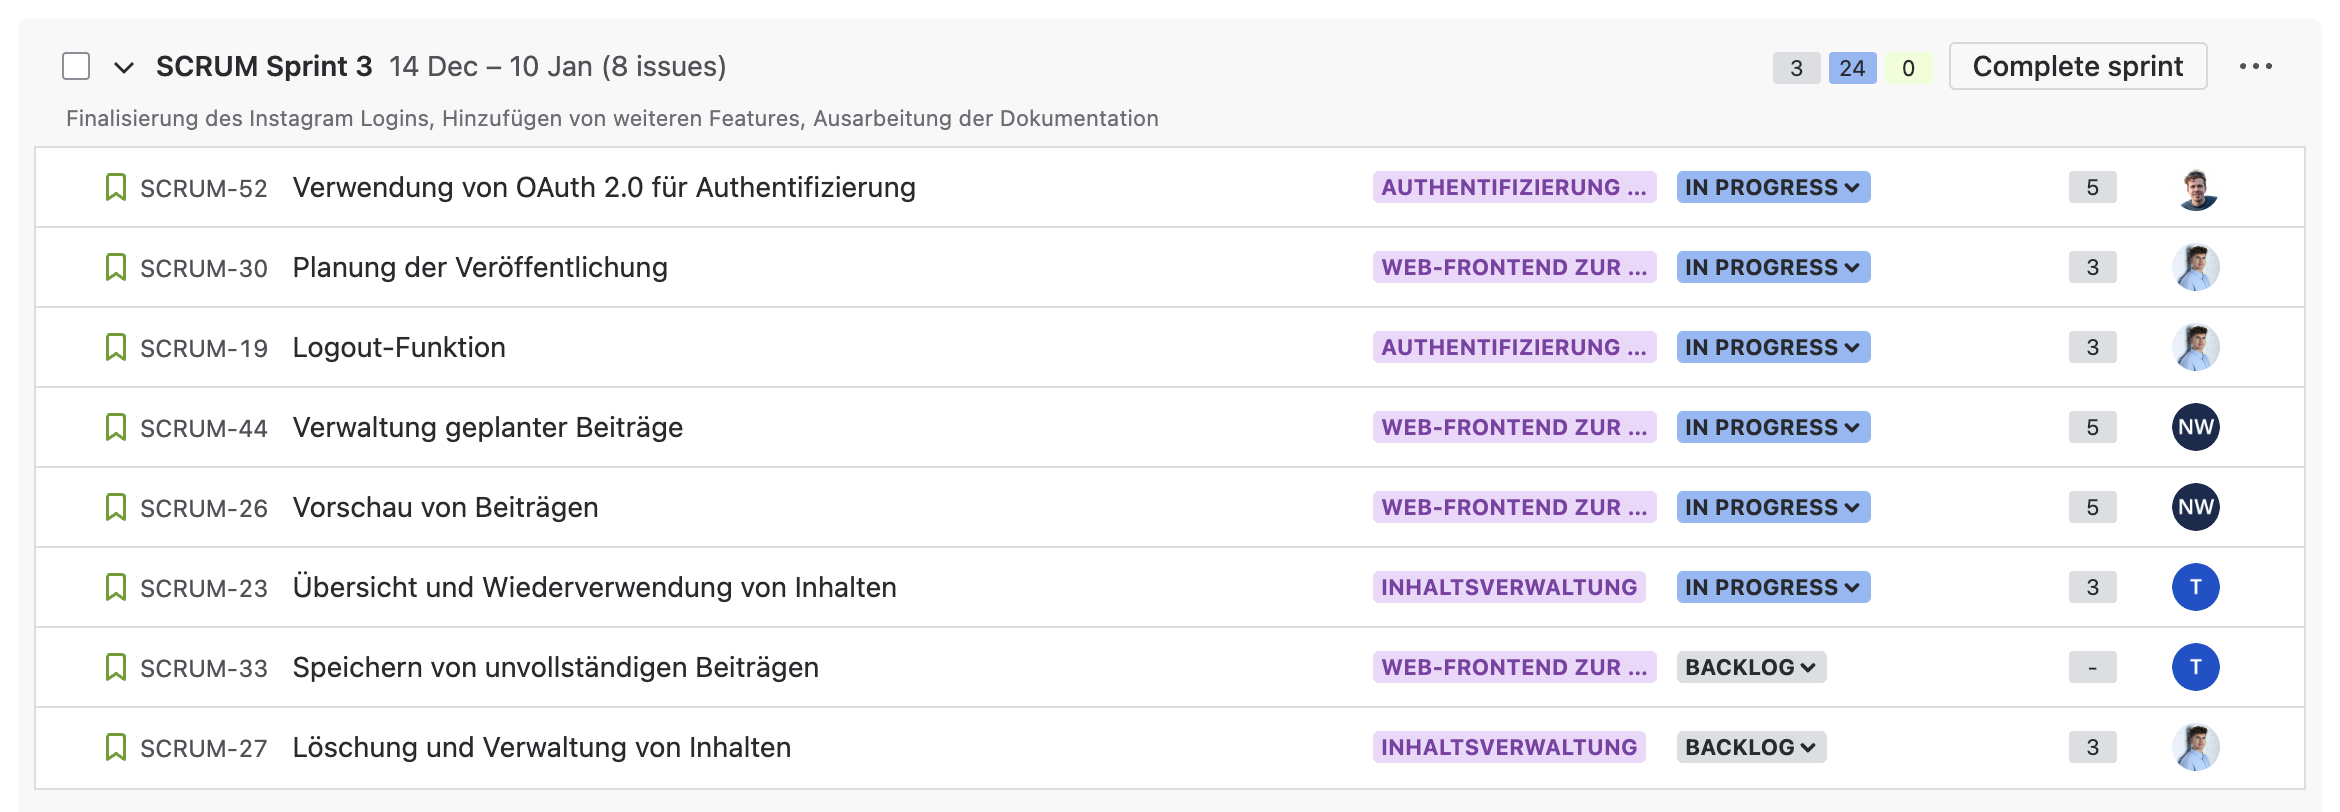
\includegraphics[width=0.8\textwidth]{graphics/sprint_3_jira.png}
    \caption{Sprint 3}
    \label{fig:fig-1}
\end{figure}

In \hyperref[fig:fig-1]{Abbildung 1} ist eine Übersicht von Sprint 3 zu sehen. Die Anzahl der Stories pro Sprint variiert je nach Komplexität und Umfang.
Die Entscheidung wie viele Stories in einen Sprint aufgenommen werden, wird im Team getroffen. Dabei wird darauf geachtet, dass die Stories in einem Sprint
realistisch umsetzbar und die Storypoints von Sprint zu Sprint annähernd gleich sind. Wird eine Storie in einem Sprint nicht fertigs gestellt, wird sie in
den nächsten Sprint übernommen.

\section{Arbeitspakete}
\label{sec:chapter1-2}
